\section{Hypothesis on the surface \& Projection} \label{sec:hypothesis_on_the_surface_and_projection}

\subsection{Global coordinates}

\cite[Sec. 2.3]{dziuk_finite_2013} It is quite convenient to use global coordinates in a neighbourhood of a hypersurface (see \cite[Sec. 2.2]{dziuk_finite_2013} for a definition of \defini{hypersurfaces}), the so-called \defini{Fermi coordinates}. This avoids working with charts and atlases when proving results and carrying out the numerical analysis. For this one introduces the \defini{oriented distance function} for $\surflisse$.

Assume in the following that $\mathcal{O} \subset \R^{3}$ is bounded and open with exterior normal $\vect{n}$ and assume that $\surflisse = \partial \mathcal{O}$ is a $\Cont^k$-hypersurface ($k \geqslant 2$). The \defini{oriented distance function} for $\surflisse$ is defined by
\[
d(x) \defeq \begin{cases}
\phantom{-} \inf\limits_{y \in \surflisse} \abs{x - y} & x \in \R^{3} \setminus \overline{\mathcal{O}} \\
- \inf\limits_{y \in \surflisse} \abs{x - y} & x \in \mathcal{O}
\end{cases}.
\]
One easily verifies that $d$ is globally Lipschitz-continuous with Lipschitz constant $1$. Since $\partial \mathcal{O}$ is a $\Cont^2$-hypersurface, it satisfies both a uniform interior and a uniform exterior sphere condition, which means that for each point $x_0 \in \partial \Omega$ there are balls $B$ and $B'$ such that
\[
\overline{B} \cap (\R^3 \setminus \Omega) = \{ x_0 \}, \quad \overline{B'} \cap \overline{\Omega} = \{ x_0 \},
\]
and the radii of $B$, $B'$ are bounded from below by a positive constant $\delta$ uniformly in $x_0$. With this observation the following lemma is {\color{red}easily proved}. 

\begin{lemme}[{\cite[Lemma 2.8]{dziuk_finite_2013}}] \label{lemme:fermi_coordinates}
We define
\[
U_\delta \defeq \ens[\big]{x \in \R^{3} \tq \abs{d(x)} < \delta}.
\]
Then $d \in \Cont^k(U_\delta)$, and for every point $x \in U_\delta$ there exists a unique point $\projvariete(x) \in \surflisse$ such that
\begin{equation} \label{eq:fermi_coordinates}
x = \projvariete(x) + d(x) \, \vect{n}(\projvariete(x)).
\end{equation}
Moreover, we have that
\[
\grad d(x) = \vect{n}(\projvariete(x)), \quad \abs{\grad d(x)} = 1, \quad \forall x \in U_\delta. 
\]
We also extend the normal constantly in the normal direction: $\vect{n}(x) = \vect{n}(\projvariete(x))$ for $x \in U_\delta$. Thus we have introduced a global coordinate system around $\surflisse$. Every point $x \in U_\delta$ can be described by its \defini{Fermi coordinates} (normal coordinates) $d(x)$ and $\projvariete(x)$ according to \Cref{eq:fermi_coordinates}.
\end{lemme}

\begin{figure}[H]
    \centering
    \tikzset{
    ddfv/.style={
        scale=1.5,
        every path/.style={thick,line join=round, cap=round},
        ptsq/.style 2 args={
          rectangle,
          fill=##1,
          inner sep=2pt,
          label={[text=##1]##2}
        },
        ptsqbord/.style 2 args={
          rectangle,
          draw=##1,
          inner sep=2pt,
          label={[text=##1]##2}
        },
        ptcl/.style 2 args={
          circle,
          fill=##1,
          inner sep=1.5pt,
          label={[text=##1]##2}
        },
        ptclbord/.style 2 args={
          circle,
          draw=##1,
          inner sep=1.5pt,
          label={[text=##1]##2}
        },
        mailleprimale/.style={
            myblue,
            fill=mylightblue
        },
        mailledualeint/.style={
            myred,
            fill=mylightred
        },
        mailledualebord/.style={
            myred,
            fill=mylightred!50!white
        },
        maillediamantint/.style={
            mygreen,
            fill=mylightgreen
        },
        maillediamantbord/.style={
            mygreen,
            fill=mylightgreen!50!white
        }
    }
}

\begin{tikzpicture}[
  ddfv
]

\def\largeur{3}
\def\ta{2.4}

% Courbe centrale
\def\f(#1){0.35*sin(1.0*#1 r)-0.15*#1}
\def\fp(#1){0.35*cos(1.0*#1 r)-0.15}

\draw[
  line width=\largeur cm,
  line cap=butt,
  line join=round,
  draw=mylightblue
]
plot[domain=0:6,samples=20,smooth] ({\x},{\f(\x)});

\draw plot[domain=0:6,samples=20,smooth] ({\x},{\f(\x)});

% Point a(x)
\pgfmathsetmacro{\ya}{\f(\ta)}
\pgfmathsetmacro{\slopea}{\fp(\ta)}
\pgfmathsetmacro{\nxa}{-\slopea/sqrt(1+\slopea^2)}
\pgfmathsetmacro{\nya}{1/sqrt(1+\slopea^2)}
\pgfmathsetmacro{\txa}{1/sqrt(1+\slopea^2)}
\pgfmathsetmacro{\tya}{\slopea/sqrt(1+\slopea^2)}

\pgfmathsetmacro{\dist}{0.6}
\pgfmathsetmacro{\xx}{\ta+\dist*\nxa}
\pgfmathsetmacro{\yx}{\ya+\dist*\nya}

\coordinate (P) at (\ta,\ya);

\draw[->, semithick] (P) -- ({\ta+1.2*\nxa},{\ya+1.2*\nya}) node[right] {$\vect{n}(\projvariete(x))$};

\def\eps{0.1}
\draw[semithick]
  (P)
  --
  ($(P)!-\eps cm!({\ta+\txa},{\ya+\tya})$)
  --
  ($($(P)!-\eps cm!({\ta+\txa},{\ya+\tya})$)!\eps cm!90:(P)$)
  --
  ($(P)!\eps cm!90:({\ta+\txa},{\ya+\tya})$)
  --
  cycle;

\node[ptcl={black}{below:$\projvariete(x)$}] at (P) {};
\node[ptcl={black}{left:$x$}] at (\xx,\yx) {};

\draw[myred, thick, <->] (P) -- (\xx,\yx) node[midway, right] {$d(x)$};

\pgfmathsetmacro{\yO}{\f(0)}
\pgfmathsetmacro{\slopeO}{\fp(0)}
\pgfmathsetmacro{\nxO}{-\slopeO/sqrt(1+\slopeO^2)}
\pgfmathsetmacro{\nyO}{1/sqrt(1+\slopeO^2)}

\pgfmathsetmacro{\distd}{\largeur/3}

\pgfmathsetmacro{\xd}{\distd*\nxO}
\pgfmathsetmacro{\yd}{\yO+\distd*\nyO}
\pgfmathsetmacro{\xdb}{-\distd*\nxO}
\pgfmathsetmacro{\ydb}{\yO-\distd*\nyO}

\draw[<->, semithick] (0,\yO) -- (\xd,\yd) node[midway, left] {$\delta$};
\draw[<->, semithick] (0,\yO) -- (\xdb,\ydb) node[midway, left] {$\delta$};

\node[myblue, above=10pt] at (1,{\f(1)}) {$U_\delta$};
\node[below] at (5.5,{\f(5.5)}) {$\surflisse$};

\end{tikzpicture}
    \caption{Strip $U_\delta$ around the hypersurface $\surflisse$ and normal coordinates $x = \projvariete(x) + d(x) \, \nu(\projvariete(x))$}
\end{figure}

\begin{prop}
The map $\fonctionens[\projvariete]{\surfpoly}{\surflisse}$ is bijective.
\end{prop}

\subsection{Sobolev spaces on surfaces}

\cite[p. 299]{dziuk_finite_2013} Let $\surflisse \in \Cont^2$ for the following. For $p \in \intervalleff{1}{\infty}$ we let $\L^p(\surflisse)$ denote the space of functions $\fonctionens[f]{\surflisse}{\R}$ which are measurable with respect to the surface measure $\d A$ ($\d A$ in connection with an integral over $\surflisse$ denotes the $n$-dimensional Hausdorff measure) and have finite norm, where the norm is defined by 
\[
\norme{f}_{\L^p(\surflisse)} \defeq \bigg( \int_{\surflisse} \abs{f}^p \d A \bigg)^{1/p}
\]
for $p < \infty$, and for $p = \infty$ we mean the essential supremum norm. The space $\L^p(\surflisse)$ is a Banach space and for $p = 2$ a Hilbert space. For $1 \leqslant p < \infty$ the space $\Cont^0(\surflisse)$ dans $\Cont^1(\surflisse)$ are dense in $\L^p(\surflisse)$. 

\begin{theo}[Poincaré’s inequality {\cite[Sec. 2.4]{dziuk_finite_2013}}]
    Assume that $\surflisse \in \Cont^3$ and $1 \leqslant p < \infty$. Then there is a constant $c$ such that, for every function $f \in \H^{1,p}(\surflisse)$ with $\int_{\surflisse} f \d A = 0$, we have the inequality
    \[
    \norme{f}_{\L^p(\surflisse)} \leqslant c \norme{\grad_{\surflisse} f}_{\L^p(\surflisse)}.
    \]
\end{theo}

\subsection{Triangulations {\cite[Sec. 4.1]{dziuk_finite_2013}}}

The smooth $2$-dimensional surface $\surflisse$ ($\partial \surflisse = \varnothing$) is approximated by a surface $\surfpoly$ which lies in the strip $U_\delta$ (see \Cref{lemme:fermi_coordinates}) and which is a Lipschitz surface. The strip can be chosen with locally varying width: see \Cref{eq:eq41}. 

We assume that the discrete triangulated surface $\surfpoly$ besides \Cref{eq:eq41} has the following properties. The surface $\surfpoly$ is the union of finitely many non-degenerate (closed) $2$-simplices in $\R^{3}$. We let $\ensprimalplat$ denote the set of these simplices:
\[
\surfpoly = \bigcup_{\primalplat{K} \in \ensprimalplat} \primalplat{K}. 
\]
The vertices $\enssomprim$ of the simplices are taken to sit on the smooth surface $\surflisse$. For $\primalplat{K}, \primalplat{L} \in \ensprimalplat$, either $\primalplat{K} \cap \primalplat{L} = \varnothing$ or $\primalplat{K} \cap \primalplat{L}$ is an $(3-k)$-dimensional side simplex ($k \in \{1, 2, 3\}$) common to both of the simplices $\primalplat{K}$ and $\primalplat{L}$. For $\primalplat{K} \in \ensprimalplat$ we denote by $\diam{\primalplat{K}}$ its diameter and by $r(\primalplat{K})$ the in-ball radius. Also, we define
\begin{equation} \label{eq:hensprimalplat_rensprimalplat}
h_\ensprimalplat \defeq \max_{\primalplat{K} \in \ensprimalplat} \diam{\primalplat{K}} 
\quad
\text{and}
\quad
r_\ensprimalplat \defeq \min_{\primalplat{K} \in \ensprimalplat} r(\primalplat{K}).
\end{equation}
We assume that the quantity
\[
\sigma_\ensprimalplat \defeq \max_{\primalplat{K} \in \ensprimalplat} \sigma(\primalplat{K})
\quad
\text{with}
\quad
\sigma(\primalplat{K}) = \frac{h(\primalplat{K})}{r(\primalplat{K})}
\]
is uniformly bounded independently of $h_\ensprimalplat$.

\begin{figure}[H]
    \centering
    \input{figures/projection_3d_courbe.tex}
    \caption{Approximation of a smooth surface by a polygonal surface : a control volume $\primalplat{K}$ and its projection $\primal{K} = \projvariete \primalplat{K}$ onto the hyperurface $\surflisse$}
    \label{fig:projection_3d_courbe}
\end{figure}

Note that, by \Cref{lemme:fermi_coordinates}, for every simplex $\primalplat{K} \subset \surfpoly$ there is a unique curved simplex $\primal{K} \defeq \projvariete \primalplat{K} \subset \surflisse$ (see \Cref{fig:projection_3d_courbe}). In order to avoid global double covering, we assume that for each point $a \in \surflisse$ there is at most one point $x \in \surfpoly$ with $a = \projvariete(x)$. This implies that there is a bijective correspondence between the triangles on $\surfpoly$ and the induced curvilinear triangles on $\surflisse$.

We assume that $\surflisse$ has only one connected component. We start with a discrete surface $\surfpoly$ contained in the variable strip $U_\delta$,
\begin{equation} \label{eq:eq41}
    \surfpoly \subset U_\delta = \ens[\big]{y + s \, \vect{n}(y) \tq \abs{s} < \delta(y),\ y \in \surflisse},
\end{equation}
where for a point $y \in \surflisse$ we set
\[
\delta(y) = \min \bigg\{ \Big( \max_{i = 1, \dots, n} \abs{\kappa_i(y)} \Big)^{-1}, \sup_{z \in \surflisse, z \not= y} \frac{L(y, z)}{\abs{y - z}} \bigg\}
\]
with the sectional curvatures $\kappa_i$ and where $L(y, z)$ denotes the geodesic distance between $y$ and $z$ on $\surflisse$ (see \cite{lee_riemannian_1997} for the definitions of \defini{sectional curvature} and \defini{geodesic distance}). 

\begin{remarque}
    We can take $\delta \defeq \min_{y \in \surflisse} \delta(y)$ which exists since $\surflisse$ is a compact manifold. 
\end{remarque}

\begin{prop}
    La courbure de la surface étant finie en tout point, il existe toujours $\delta$ pour que $U_\delta$ ne s'auto-intersecte pas. Nous faisons l'hypothèse
    \begin{itemize}
        \item[$\mathcal{H}$] Il existe $h$ suffisamment petit tel que $\surfpoly \subset U_\delta$. 
    \end{itemize}
\end{prop}

\begin{prop}
One can show that each point $x \in U_\delta$ can be uniquely projected onto the smooth surface, yielding the decomposition
\[
x = \projvariete(x) + d(x) \, \vect{n}(\projvariete(x)), \quad x \in U_\delta,
\]
with $\projvariete(x)$ the orthogonal projection of $x$ onto $\surflisse$ and $d(x)$ the oriented distance between $x$ and $\surflisse$. 
\end{prop}

\begin{figure}[H]
    \centering
    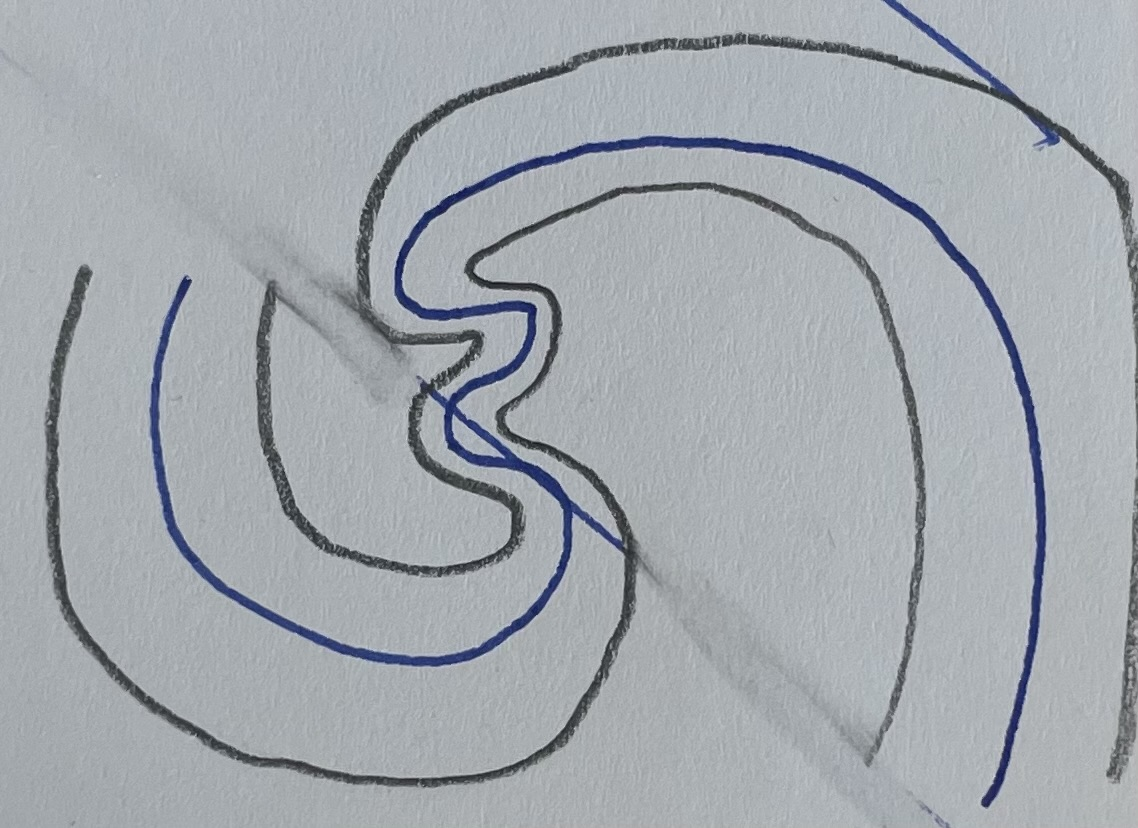
\includegraphics[width=0.5\textwidth]{img/strip_varying.jpeg}
    \caption{$\delta(y)$}
\end{figure}

\begin{theo}
\[
\primal{K} \defeq \projvariete \primalplat{K}
\quad
\mailleduale{K} \defeq \projvariete \mailledualeplate{K}
\quad
\diamant{D} \defeq \projvariete \diamantplat{D}
\]
\[
\ensprimal \defeq \ens[\big]{\primal{K}}
\quad
\ensdual \defeq \ens[\big]{\mailleduale{K}}
\quad
\ensdiamant \defeq \ens[\big]{\diamant{D}}
\]
\end{theo}